\section{Discussion}

\subsection{Nitrite Investigations}
We have found that use of both disposable and reusable gold electrodes are suitable for measuring nitrite concentrations in solution as mentioned previously in background. (Our chosen nitrite concentrations reflect the normal physiological levels and expected elevation in septic patients.) Therefore, DPV is found to be a reliable method of measuring the electrochemical activity of nitrite in solution. However, using our parameters, each measurement takes 405s. This may prove a challenge for both real-time monitoring and in the clinical setting.\\\\
DPV voltammograms from nitrite experimentation reveals a common peak where the peak current recorded increases with higher concentrations of nitrite, across all experiments, between 0.7 and 0.8 V, which is as expected from literature \cite{article}. Small peaks corresponding to an unknown species was reliably detected at 0.2 V in PBS only experiments, but were not present in albumin experiments. Increased noise and smoothing may have eliminated this peak. We hypothesise that small peaks may have resulted from oxygen impurities in solution.\\\\ 
The albumin experiments showed that at low nitrite concentrations (below 16 µM), the sensitivity is comparable to results without albumin. However, at higher nitrite concentrations, the sensitivity increases to 7nA µM-1, with a marked change in the calibration curve (Figure 8), suggesting interactions between the nitrite and the albumin. Detected current was greater overall in albumin experiments compared to without albumin. This contradicts the hypothesis that albumin adsorbs onto the electrode surface, interfering with the electrode's ability to detect nitrite.

\subsection{Hydrogen Peroxide Investigations}
To perform hydrogen peroxide electrochemical detection using the microneedles platform, we have conducted chronoamperometry, an electrode calibration experiment, with gold electrodes over a range of hydrogen peroxide concentrations. The calibration process was facilitated by the reactions between hydrogen peroxide and Prussian blue PEDOT:PSS-PB complex, as shown in \autoref{eqn:h2o2redox1} and \ref{eqn:h2o2redox2}. Following the amperometry, we performed coulometry to validate the experimental concentration and amplify the signal and reduce the noise from the raw data. \\\\It is observed that under low hydrogen peroxide concentrations, specifically below 100uM, there are significant percentage differences between the experimental and theoretical concentration values. In the future, a more discreet selection of the equipment for liquid transferring is critically required, thus an improvement of the experimental accuracy can be accomplished. Also, a non-linearity condition was observed in the current vs time plot under high hydrogen peroxide concentrations, especially when $c>300$uM. By performing quantitative analysis based on \autoref{eqn:h2o2redox2} and the actual amount of reactants involved in the experiment, an approximation of hydrogen peroxide concentration limit was found at 280uM, indicating an excess of the hydrogen peroxide concentration would result in insufficient PB to react with H$_{\text{2}}$O$_{\text{2}}$. 


\subsection{Lactate Investigations}
The differences in behaviour of the current concentration behaviour conveyed in \autoref{fig:lactate_result}(b) and (c), can be explained by lactate oxidase enzyme kinetics.\\\\
The linear range suggested by the data is 0.0-2.0mM lactate. The current is approximately purely dependent on the lactate concentration. The electron flow is indicative of the reaction rate. 
%In this region of the graph, purely dependent on lactate concentration
% enzyme concentration or enzyme ability to allow binding has no effect on the sensing abilities.
After 2.0mM, the reaction rate can be seen as starting to plateau, whilst there is no limit in detection observed in the concentration range tested, it can be assumed that it is being approached. The non-linear behaviour of the relationship is therefore due to enzyme kinetics.\\\\
\begin{figure}[H]
    \centering
    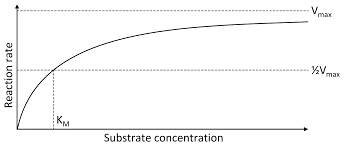
\includegraphics{img/lactate_discussion_1.png}
    \caption{Michaelis-Menten Kinetic plot of enzyme substrate reactions. }
    \label{fig:lactate_discussion}
\end{figure}
Michaelis Menten equations for reaction velocity \cite{johnson2011original}:
\begin{equation}
    E + S \xrightleftharpoons[k_{\text{off}}]{k_{\text{on}}} ES \xrightarrow{k_{cat}} E+P \quad \quad v = \frac{V_{max}[S]}{K_{M}+[S]}
\end{equation}
Enzyme kinetics can be defined partially by their Michaelis constant, Km, which describes the lactate concentration at which the current is half of that of the detection limit as seen in \autoref{fig:lactate_discussion}. In the Michaelis- Menten model, $v$ represents reaction velocity. We can take current to be proportional to $k_{cat}$, and, hence, proportional to the velocity of the H\textsubscript{2}O\textsubscript{2} production. From the Michaelis-Menten equation, as $V_{max}$ and Km are constants, the plot is hyperbolic and at higher concentrations, we can expect a decreased climb in velocity; Our calibration plot is in accordance to this. Since Michaelis-Menten kinetic models requires that immobilisation of the LOX in the matrix have no effect on its affinity for lactate, we instead approximate a value for $K_{m}$ by calculating an apparent constant $K_{m[app]}$. We can approximate $v_{max}$ $4.04\times10^{-6}$ A based on our calibration curve. This then gives a $K_{m[app]}$ proportional to the concentration where a current of $2.02\times 10\textsuperscript{-6}$A would be observed at approximately 1.0mM.\\\\
We can conclude that the Nafion membrane modified sensor is therefore useful at detecting concentrations in the range experimented. Although readings plateau in the upper range of lactate concentrations, since a patient is septic anywhere in this range- the same measures (i.e administration of antibiotics) would be taken whether the patient exhibits levels in the 3.5-4.5mM range as would be taken if levels are beyond 4.5mM.  
\subsection{Aptamer Modelling}
In this study, we have developed a novel numerical inverse laplace algorithm capable of decomposing multi-exponential chronoamperometric current signals. We show this algorithm is able to resolve rate constants up to a resolution of $k_{A} = 200s^{-1}$ and $k_{AT} = 400s^{-1}$, on simulated signals with realistic noise levels. Accurate estimates were also obtained for the coefficients, showing the accuracy of the algorithm in obtaining target concentration, [T]. These values of rate constants are closer compared to the $k_{A} = 125s^{-1}$ and $k_{AT} = 500s^{-1}$ quoted in Plaxco's study \cite{arroyo2018subsecond}.\\\\
In parallel, we develop a coarse-grained model of aptamers by assuming it as a freely-jointed chain to gain insight into the physical effects of target binding. We generate length probability distributions, and assess how the probability of a collision event $P(L<1.5nm)$ varies with Aptamer length. These estimates correlate with aptamer modelling studies in the literature \cite{uzawa2010mechanistic,uzawa2009length}.\\\\